\section{Visual Design}

\lm{With the design consideration (introduced in Section~\ref{}), we design a visual analytic system...} \lm{Show a overview figure, to introduce the relationship between multiple views}
% overview of the data. Encode information but also allow users to set multiple criteria (\textit{C1}). Support users to slice the data by different domains.}
% Semantic understanding of social characteristics.


\subsection{Data-driven Profile Visualization}

Glyph-based visualization~\cite{borgo2013glyph} is the form of visual design to compose multivariable into a collection of unified visual symbols, known as a glyph. A glyph is intended for quick understanding and aligned comparison. \lm{Dual glyphs are designed, to illustrate the information of individual from two different perspectives, i.e., detailed inspection of individuals and efficient comparsion over multiple individuals.} 

\paragraph{Star-like Glyph} \lm{To compare over multiple individuals, a star-like glyph is designed to summary each individual, to ease the comparison by common cooridnating configurations....}

\paragraph{Cartoon Glyph} ... Among glyph design, Chernoff Face~\cite{chernoff1973use} represents data variables by the different features of a cartoon face. Following the idea of Chernoff Face, we design a type of glyph, a graphical representation of people with specific individual characteristics. The idea behind using faces is that humans easily recognize faces and notice small changes without difficulty (\textit{C1}). Those visual profiles are intended for intuitive visual understanding, from abstract to concrete and semantic understanding, to support users to target the interested individual groups effectively.

Figure~\ref{fig:design_profile} shows the legend for the user profile. The eight domains are encoded by visual symbols and organically organized in a human figure. There are basically three types of variables to drive the figure, i.e., the numeric, categorical and boolean ones. For numeric attributes such as income and education levels, visual symbol keeps consistent design but with changing visual variation, such as size, thickness. For the categorical attributes such as job, visual symbols are designed separately for better semantic meaning. For the boolean attribute like car, house, a symbol is designed to indicate its existence. With this consideration, the domains are designed as follows:

% For numeric attributes. 

% By different composition, stimulus pattern which has the abstract demographic measurement of individuals.

\begin{itemize}
\item \textbf{Gender} the gender is visually mapped to the hairstyle of the avatar. 
\item \textbf{Age} age is implied by the decoration on the hair. For the elder above 70, the hair is dyed to gray. For the youth beneath 18, a hair decoration is adapted for the different hairstyles of girls and boys.
\item \textbf{Education} The thickness of eyeglasses is used to indicate the different levels of education.
\item \textbf{Job} The clothes is designed to imply the job of the individual. There are 9 types of clothes.
\item \textbf{Belongings} for real estate, car, residential license are considered as the belongings to the individual, so we design each of them as an add-on decoration to imply whether the individual has it or not.
\item \textbf{Income} a money symbol is used to represent the income, whose size encodes the income level. The more money an individual earns, the larger the symbol is.
\end{itemize} 

\begin{figure}[htb!]
 \centering % avoid the use of \begin{center}...\end{center} and use \centering instead (more compact)
 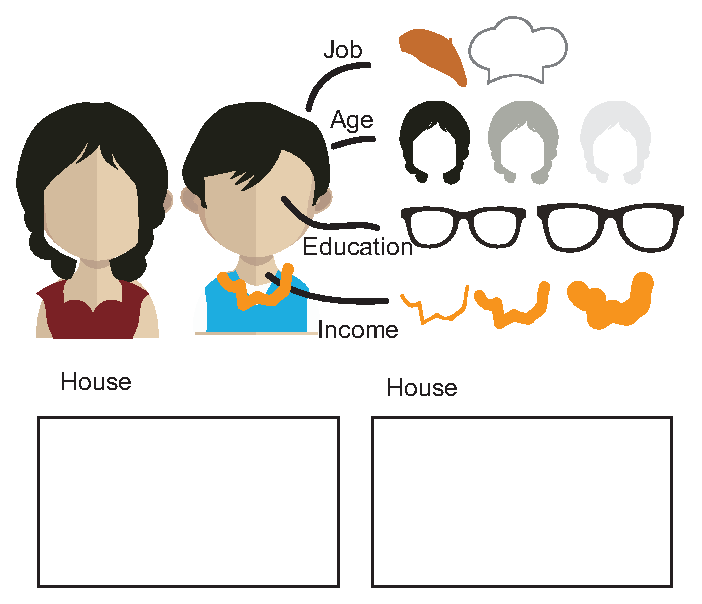
\includegraphics[width=\columnwidth]{pictures/design_profile}
 \caption{Design Profile: the eight characteritical domains are encoded and organized in an organic human figure.}
 \label{fig:design_profile}
\end{figure}

With the visual mapping, the profile varies from individual to individual. By concretizing the attributes which otherwise is too abstract to percept, users can scan and search for interesting target effectively. Figure~\ref{fig:div_example} lists the figures with the top 10 largest population in some job. The textual number beneath indicates the population. It is found that the majority of workmen earn a low salary and most of them have no residential license. On the contrary, for the officers, all of them have the residential license and most of them have a house. Some of the retired people are in old age. Most of the managers are at undergraduates, even graduates. 



% \begin{figure}[htb!]
%  \centering % avoid the use of \begin{center}...\end{center} and use \centering instead (more compact)
%  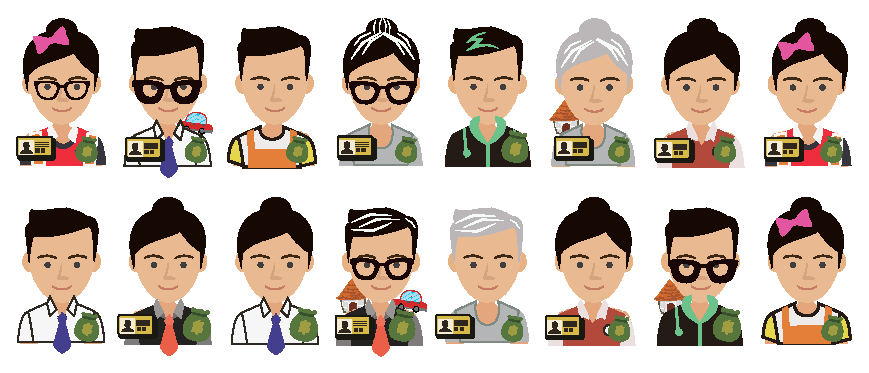
\includegraphics[width=\columnwidth]{pictures/design_div}
%  \caption{Diverse Profile}
%  \label{fig:div_profile}
% \end{figure}

 
\begin{figure}[htb!]
 \centering % avoid the use of \begin{center}...\end{center} and use \centering instead (more compact)
 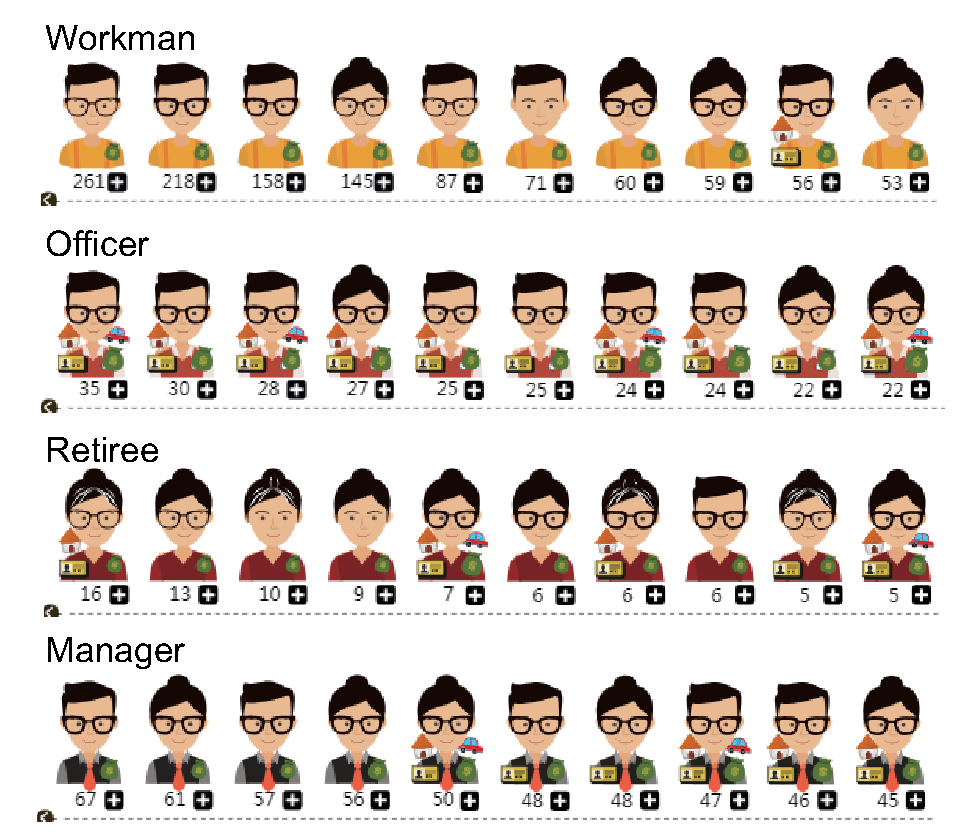
\includegraphics[width=\columnwidth]{pictures/design_example}
 \caption{Representative figures with the top 10 largest population in four jobs}
 \label{fig:div_example}
\end{figure}

\subsection{t-SNE Projection of Individuals}



% \begin{figure}[htb!]
%  \centering % avoid the use of \begin{center}...\end{center} and use \centering instead (more compact)
%  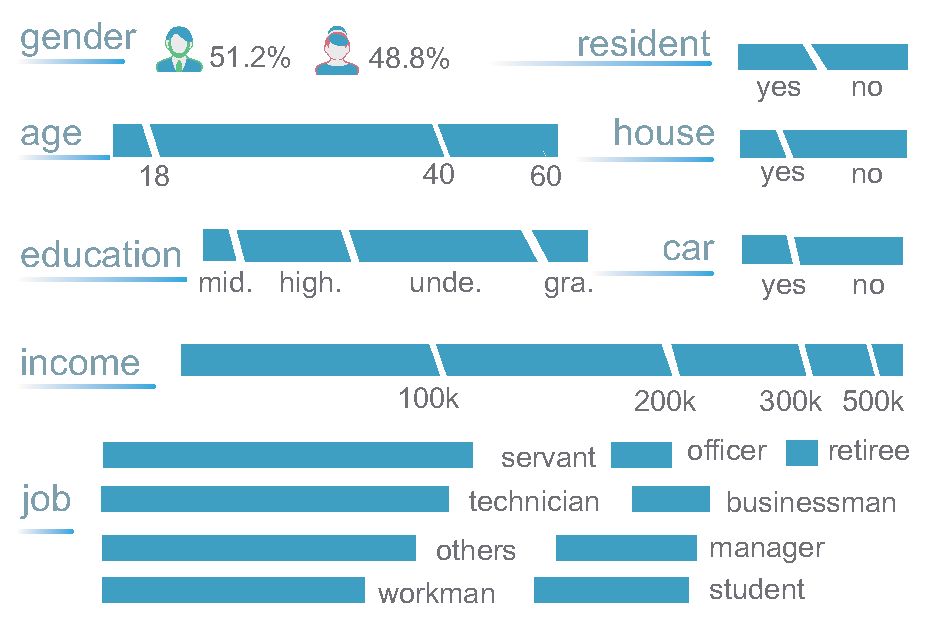
\includegraphics[width=0.7\columnwidth]{pictures/data_overview}
%  \caption{Overview of Multiple Variables}
%  \label{fig:figoverview}
% \end{figure}

In our case, each individual can be denoted as a vector $x_i$ with eight factors, and we get high dimensional data set $X={x_1, x_2, ..., x_n}$. The dimensionality reduction techniques are to preserve the local structure of high dimensional data in low dimensional space, which are efficient approaches to provide a good overview of the multivarible individuals (\textit{C2}). We adapt t-SNE project~\cite{maaten2008visualizing} to project $X$ as two-dimensional dots $Y={y_1, y_2, ..., y_n}$. One of steps in t-SNE is to compute the conditional probabilities to represent the similarity based on the distance between high dimenional datapoints. The conditional probability $p_{j\mid i}$ between $x_j$ and $x_i$ is given by:

\begin{equation}
p_{j\mid i} = \frac{exp({\left \| x_i - x_j \right \|}^2/2\alpha_i ^{2})}{\sum _{k\neq i}exp({\left \| x_i - x_k \right \|}^2/2\alpha_i ^{2})}
\end{equation}

where $\alpha_i$ is the variance of the Gaussian that is centered on $x_i$. Specifically in our context, the high-dimensional Euclidean distances $\left \| x_i - x_j \right \|$ between $x_i$ and $x_j$ needs to be adpated the numerical and categorical characteristics. Characteristics such as age, income, are numerical and comparable, so the difference exactly explains when they are different. But the other characteristics, i.e. job, real estate, car, residential, are ordinal. There is not the numeric order. For example, the job distance from a manager to a businessman and a workman is not comparable, which is considered the same distance, i.e., set to 1. 

% So $\left \| x_i - x_j \right \|$ is adapted as following:

% \begin{equation}
% \left \| x_i - x_j \right \| = 
% \left\{\begin{matrix}
% 0, f_{pi} \equiv f_{pj} \Lambda f_{p} \epsilon \{Gender, Residence, Estate, Car, Job\} \\ 
% 1, f_{pi} \not\equiv f_{pj}  \Lambda f_{p} \epsilon \{Gender, Residence, Estate, Car, Job\} \\ 
% \left \| f_{pi} - f_{pj} \right \|, f_p \epsilon\{Age, Education, Income, \}
% \end{matrix}\right
% \end{equation}

As Figure~\ref{fig:tsne}shows, all 21435 volunteers are embedded in the 2D view, where the closer two dots are, the more similar they are in the eight characteristics. Figure~\ref{fig:tsne} exemplifies four features groups of dots in a neighbor. 

Multiple views of abstract view, t-SNE protection, and semantic data-driven profile visualization are coordinated in a Cross-filter machinesm~\cite{Weaver2010}. It allows end-users to interactive drill-down into individuals with interested characteristics from multiple perspectives(\textit{C3}). Starting from the abstract criterion constraints, the scope of interest is narrowed down to individuals with(out) certain characteristics. And then further cross-filtering with semantically visual profiles can be performed to check the combination of 8 characteristical variables. 

\begin{figure}[htb!]
 \centering % avoid the use of \begin{center}...\end{center} and use \centering instead (more compact)
 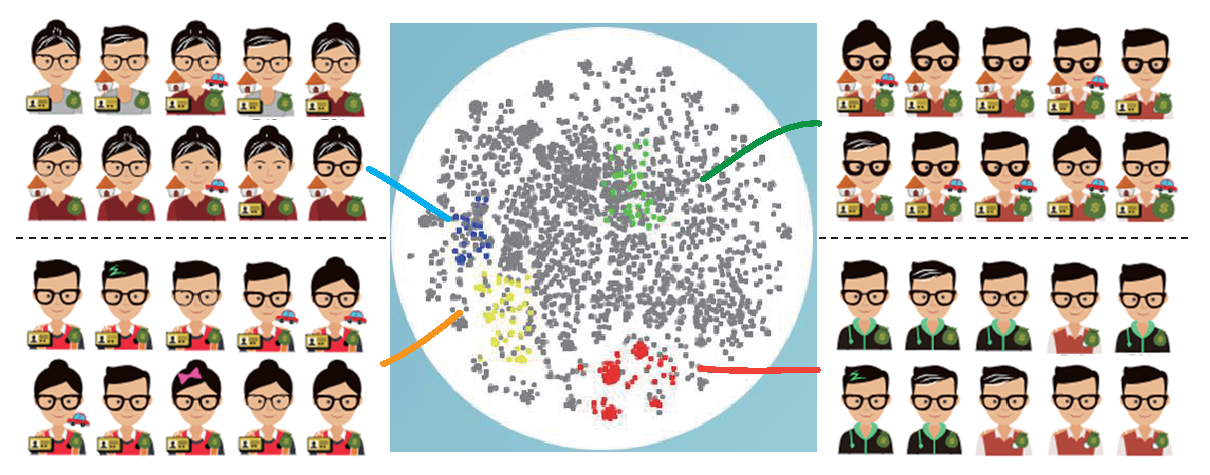
\includegraphics[width=\columnwidth]{pictures/tsne}
 \caption{t-SNE project with four groups of the interest: (a) t-SNE project }
 \label{fig:tsne}
\end{figure}

\subsection{2.5D Spatial Visualization}
\label{subsec:25D}


Embedding multiple variables in the spatial map is a challenging problem. Distorting 2D spatial for better space usage, such as the partial route embedding~\cite{sun2016embedding} is an effective method when there are a few local foci. When it comes to the global visualization, there is always a trade-off between occlusion-free and the compact spatial perception. Following the idea of stacking 2.5D space design~\cite{Tominski2012_stacking}, the space in this work is embedded in 2.5D space, to relax the z-axis for additional abstract information encoding.

Figure~\ref{fig:2.5D}(a) shows the 2.5D visualization. The spatial map consists of Traffic Analysis Zone (TAZ), which is the unit of geography holding a certain number of people. For the 2.5D, each TAZ is grown as a prism whose height and color are developed to encode abstract information, e.g., the occurrence of visiting. With difference encoding choices, it is capable to visualize the correlation between spatial and different attributes (\textit{C4}). For example, in Figure~\ref{fig:2.5D}(a), prisms' height and color both encode the ratio of none-routine trips (such as go entertainment, go hospital, etc.) in the whole. For better 3D visual perception, lighting is turned on. Also, a lid is laid on the top of each prism to clearly bound its extent at the z-axis. 

\begin{figure}[htb!]
\centering
\subfigure[]{
\resizebox*{9cm}{!}{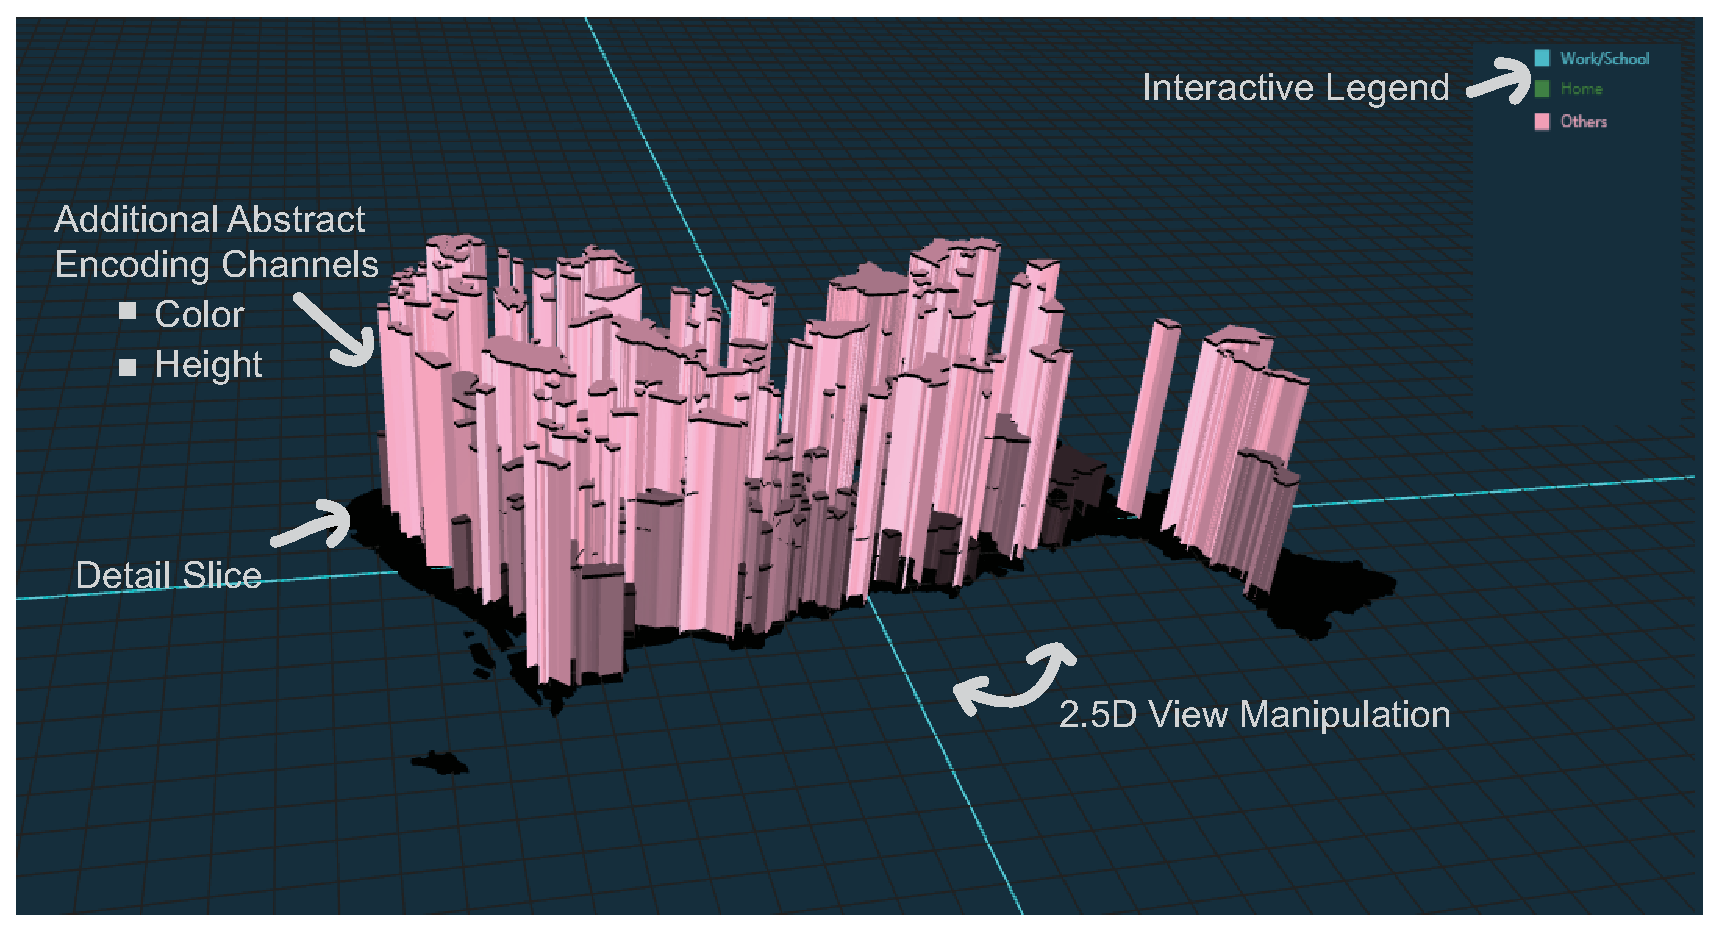
\includegraphics{pictures/space1.eps}}}\hspace{5pt}
\subfigure[]{
\resizebox*{9cm}{!}{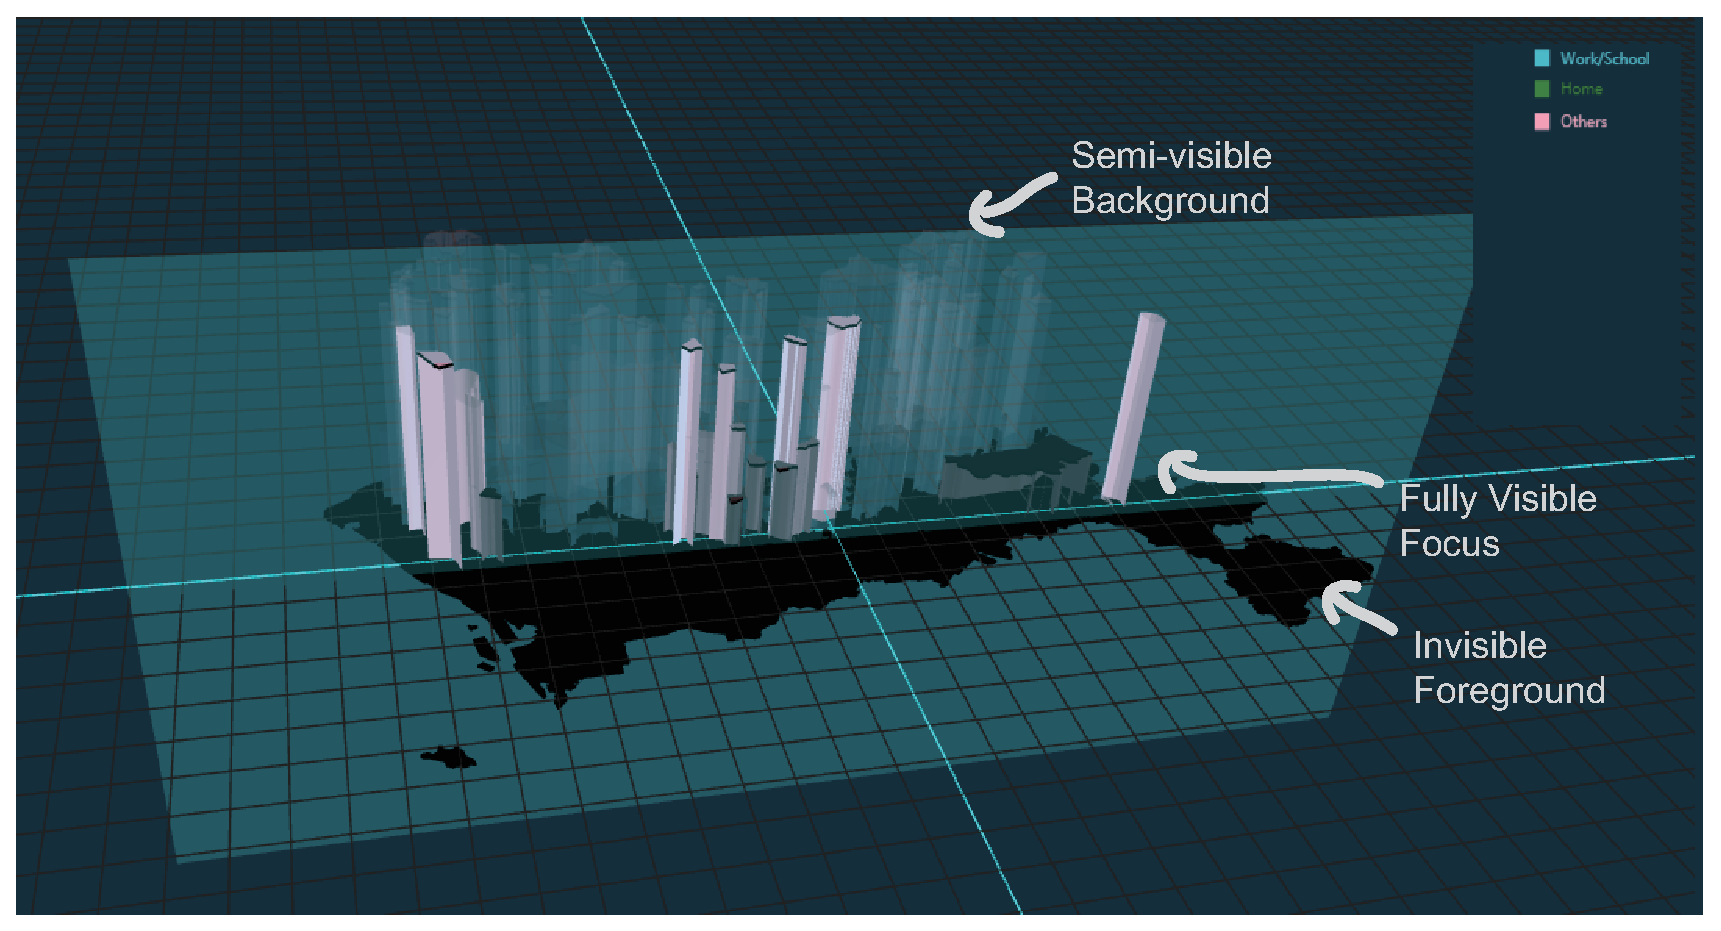
\includegraphics{pictures/space2.eps}}}\hspace{5pt}
\caption{2.5D Spatial Visualization: (a) 2.5D spatial visualization with z-axis to encode addition information; (b) detail slicing in 2.5D space.}
\label{fig:2.5D}
\end{figure}

Several interactions are integrated into the spatial view to alleviating the occlusion problem (\textit{C5}). The manipulation of 2.5D view supports users with rotate, zoom, pan operations, which are so continuously flexible that users probably find a suitable observing point. In the cases where occlusion is inevitable, an interaction named as \textit{Detail Slicing} is developed, as Figure~\ref{fig:2.5D}(b) shows. Detail Slicing is the operation to put a cross-section in the 2.5D space to expose the TAZ inside. To contextualize the cross-section, TAZs are visually adapted according to the intersection by ray casting. The TAZ in the foreground will be hidden, the intersected TAZs will be fully visualized and the ones in the background will be in semi-transparency.
% Brunch of TAZ with similar visiting pattern and purpose are grouped by a heuristic DB-Scan Algorithm in the context of TAZ. From a center TAZ, walk to neighbor TAZ to check whether aggregation or not. The aggregated TAZ brunch indicates the region visiting the group of people in the same purpose, which is often the popular traveling places. The TAZ brunch is visualized...

 To compare the mobility patterns across different groups of people, a Small Multiple dock is used to reserve the ever explored interesting result (Figure~\ref{fig:teaser}(f)). To simply the comparison over spatial distribution, the snapshot is also rendered in the 2.5D space, which maintains the same interactions as the main 2.5D space does.

 % In this view, it supports end-users to directly manipulate the space, e.g., zooming, panning, etc. Also, detail information about the visiting can be checked by direct clicking on the TAZ. 
